\documentclass{beamer}
\usepackage{etoolbox}\newtoggle{printable}\togglefalse{printable}
\usetheme{CambridgeUS}
\usepackage{listings}
\usepackage{algpseudocode}
\pdfmapfile{+sansmathaccent.map}
\graphicspath{ {Images/} }

\title{Comp230 Networking component}
\author{Alastair Rayner}
\date{\today}

\begin{document}

\maketitle

\begin{frame}{About the Networking Component}
	\begin{itemize}
		\item For my Comp230 collaborative project I chose to work with a BA team and help them with the networking component of their game.\pause
		\item I have been primary focusing on the lobby system. \pause
		\item Their game is being built in Unity. \pause
		\item I have been working on a lobby GUI which was based of a Unity lobby template. \pause
		\item As well as helping the programmers in the BA team integrate other networked functionality such as: \pause
		\begin{itemize}
			\item Player Movement. \pause
			\item Player Health. \pause
			\item Spawnable Items (I.e. bullets)
		\end{itemize}
	\end{itemize}
\end{frame}

\begin{frame}{The Market, Target Audience and Unique Selling points}
	\begin{itemize}
		\item There is a large audience when it comes to multilayer games, as a lot of AAA titles that have come out in the last few years have some sort of multiplayer aspect. \pause
		\item The target audience would be people who like to play video games with their friends, especially at LAN parties etc. \pause
		\item Unique Selling Points \pause
			\begin{itemize}
				\item This type of turn-based first person shooter is not very common. \pause
				\item Having a lobby system that allows players to matchmake easily. \pause
				\begin{itemize}
					\item This allows for quick easy gameplay.  \pause
				\end{itemize}
				\item  Online matchmaking \pause
				
			\end{itemize}
		\item Having a multiplayer aspect to the game can help with advertising.
	\end{itemize}
\end{frame}

\begin{frame}{Scope}
	\begin{itemize}
		\item Unity has quite a high level networking architecture already built in it.  \pause
		\item This meant that I didn't have to program very low level networking stuff and worry about security etc. \pause
		\item This made the scope of this component manageable for this time-frame. \pause
		\item However there is still a lot to be improved upon.
	\end{itemize}
\end{frame}

\begin{frame}{Images of the Lobby GUI}
	\begin{itemize}
		\item Lobby Menu. \pause
		\item 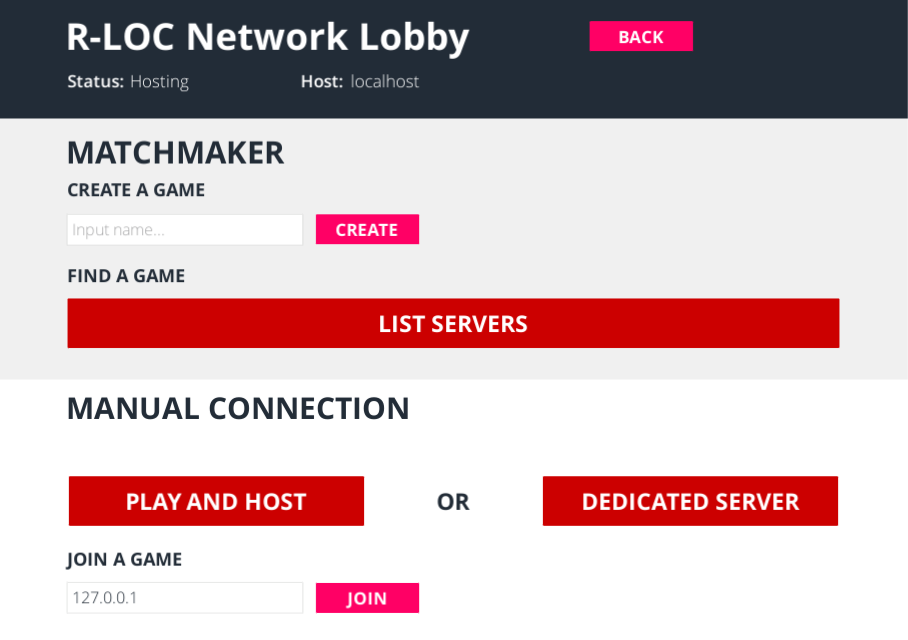
\includegraphics[width=8cm]{LobbyGUI} \pause
		\item Currently the Online Matchmaking isn't working.
	\end{itemize}
\end{frame}

\begin{frame}{Images of the Lobby GUI}
	\begin{itemize}
		\item Lobby Setup \pause
		\item 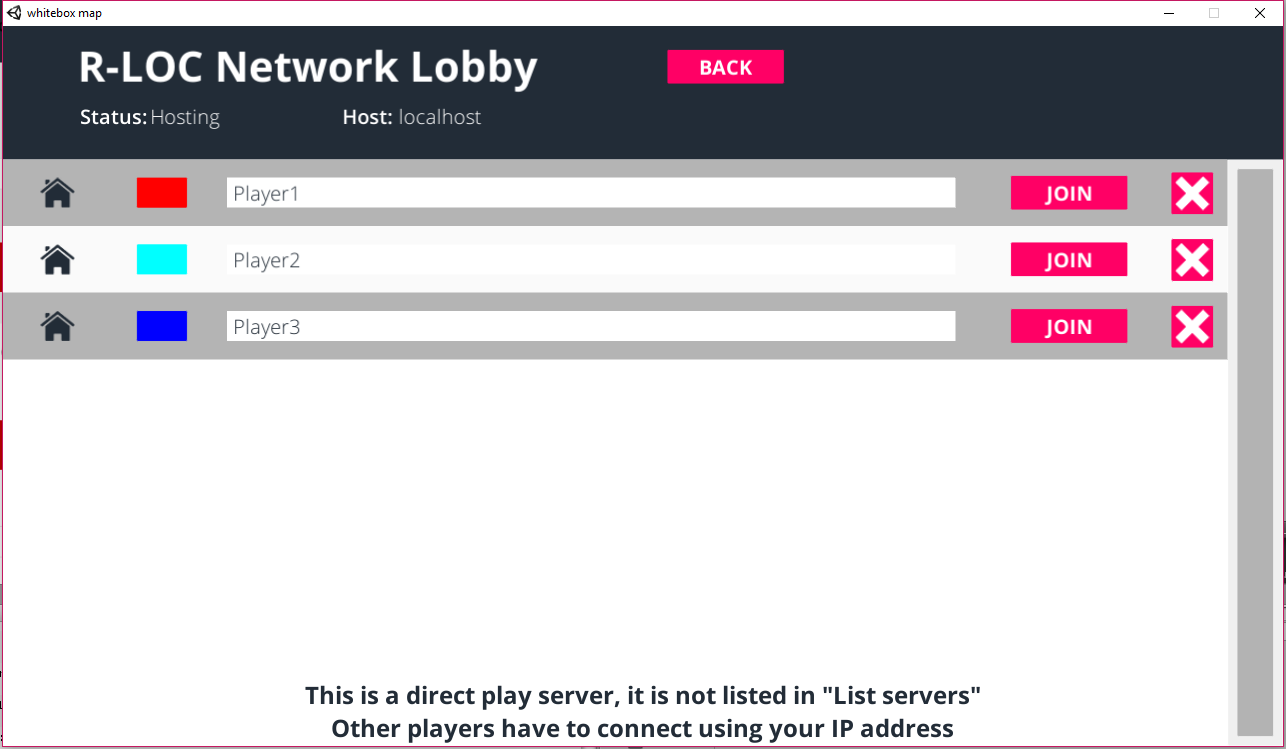
\includegraphics[width=8cm]{LobbySetup}
	\end{itemize}
\end{frame}

\begin{frame}{Networking Video Demo}
	\begin{center}
	Demo of working lobby and networked player movement.
	\par
		\url{https://www.youtube.com/watch?v=fUtDHb1e6x8&feature=youtu.be}
	\end{center}
\end{frame}

\begin{frame}{Moving Forward into Production}
	\begin{itemize}
		\item Lobby Menu GUI improvements. \pause
		\item Aim to get online matchmaking working. \pause
		\item Player is able to choose different types of units and select a map.
	\end{itemize}
\end{frame}
\begin{frame}{Questions?}
\begin{center}
\textbf{Questions?}
\end{center}
\end{frame}

\end{document}
